\section{Esercitazione 1}

\subsection{Librerie di base per il calcolo seriale in Algebra Lineare Numerica (BLAS)}

Gran parte dei problemi del calcolo scientifico ed ingegneristico richiede di risolvere uno o più problemi dell'algebra lineare numerica (ALN):

\begin{itemize}

	\item Risoluzione di sistemi lineari;
	\item Risoluzione di problemi ai minimi quadrati;
	\item Ricerca di autovalori e/o autovettori;
	\item Calcolo della SVD (valori e vettori singolari);

\end{itemize}

Inoltre, la risoluzione di questi problemi è generalmente una percentuale considerevole del costo computazionale totale richiesto per la risoluzione del problema globale; questo costo si traduce spesso in ore o giorni di tempo-macchina impiegato. Dunque, implementare in modo efficiente gli algoritmi che risolvono i problemi dell'algebra lineare numerica è estremamente importante dal punto di vista applicativo ed è anche per questo che trattiamo questo caso più approfonditamente.
Un secondo motivo è dovuto al fatto che esistono in rete delle librerie che rappresentano lo stato dell'arte per questi problemi e sono molto ben costruite anche dal punto di vista della implementazione e distribuzione del software numerico: BLAS, LAPACKe ATLAS (disponibili al sito www.netlib.org/blas , /lapack e /atlas).

Gli algoritmi di algebra lineare numerica hanno in comune un insieme relativamente piccolo e stabile di operazioni di base, che svolge la quasi totalità dei calcoli necessari negli algoritmi di ALN. Questo fatto giustifica lo sforzo di creazione di una libreria che implementi queste funzione di base. La libreria BLAS è organizzata in tre livelli:
operazioni che lavorano su vettori e producono uno scalare  (es. il prodotto interno, o scalare, tra due vettori colonna: v' * w), operazioni tra vettori e matrici o che comunque producono una matrice (es. il prodotto esterno tra due vettori colonna: v * w'), operazioni tra matrici (es. il prodotto di due matrici).

Un vantaggio rilevante di aver creato la BLAS è che questa può essere ottimizzata per ogni singola macchina ed in questo modo gli algoritmi di ALN possono diventare ``portabili'' anche dal punto di vista delle prestazioni di calcolo e non solo da quello della sintassi, semplicemente chiamando le routines della BLAS ove possibile.

Ora, ha senso chiedersi se le operazioni di livello 1, 2 o 3 raggiungono le stesse prestazioni di calcolo. Lo vediamo implementando lo stesso identico algoritmo, il prodotto di due matrici C = A * B, in tre modi diversi, corrispondenti all'utilizzo esclusivo di operazioni di livello 1, di livello 2 e di livello 3.

\begin{figure}[ht!]
\centering
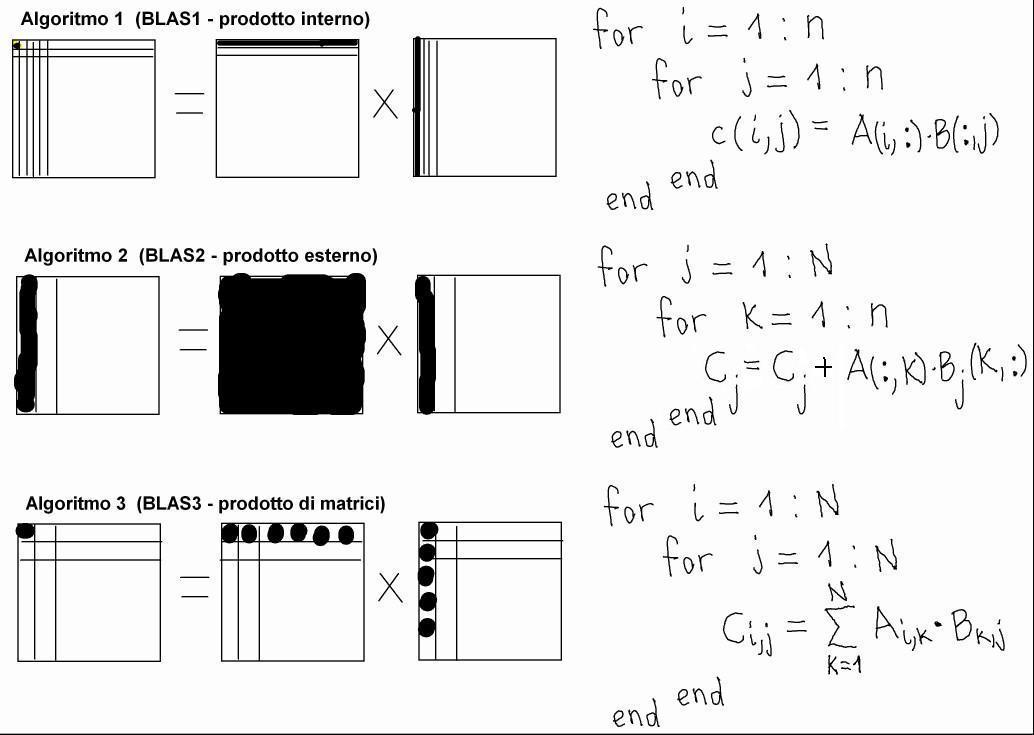
\includegraphics[width=130mm]{images/implementazioni_prodotto_di_matrici.jpg}
\caption{Algoritmi BLAS}
\label{overflow}
\end{figure}